\documentclass{article}
\usepackage{tikz}
\usetikzlibrary{arrows,automata}

\begin{document}

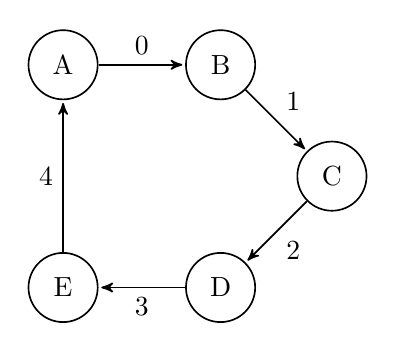
\begin{tikzpicture}[->,>=stealth',shorten >=1pt,auto,node distance=2cm,
                    semithick]
  \tikzstyle{every state}=[fill=white,draw=black,text=black]

  \node[state] (A) {A};
  \node[state] (B) [right of=A] {B};
  \node[state] (C) [below right of=B] {C};
  \node[state] (D) [below left of=C] {D};
  \node[state] (E) [left of=D] {E};

  \path (A) edge node {0} (B)
        (B) edge node {1} (C)
        (C) edge node {2} (D)
        (D) edge node {3} (E)
        (E) edge node {4} (A);
\end{tikzpicture}

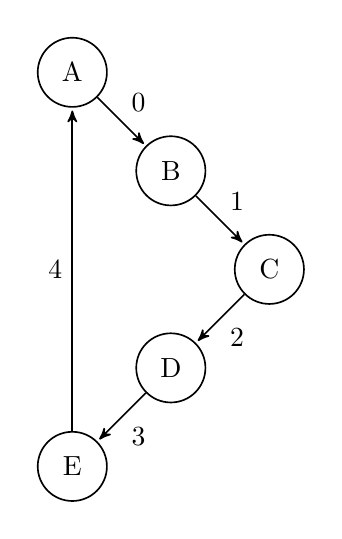
\begin{tikzpicture}[->,>=stealth',shorten >=1pt,auto,node distance=2cm,
                    semithick]
  \tikzstyle{every state}=[fill=white,draw=black,text=black]

  \matrix[row sep=1em, column sep=1em] {
    \node[state] (A) {A}; & & \\
    & \node[state] (B) {B}; & \\
    & & \node[state] (C) {C}; \\
    & \node[state] (D) {D}; & \\
    \node[state] (E) {E}; & & \\
  };

  \path (A) edge node {0} (B)
        (B) edge node {1} (C)
        (C) edge node {2} (D)
        (D) edge node {3} (E)
        (E) edge node {4} (A);
\end{tikzpicture}

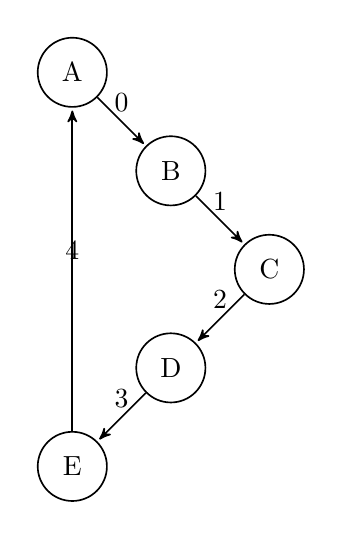
\begin{tikzpicture}[->,>=stealth',shorten >=1pt,auto,node distance=2cm,
                    semithick]
  \tikzstyle{every state}=[fill=white,draw=black,text=black]

  \matrix[row sep=1em, column sep=1em] {
    \node[state] (A) {A}; & & \\
    & \node[state] (B) {B}; & \\
    & & \node[state] (C) {C}; \\
    & \node[state] (D) {D}; & \\
    \node[state] (E) {E}; & & \\
  };

  \path (A) edge node[above] {0} (B)
        (B) edge node[above] {1} (C)
        (C) edge node[above] {2} (D)
        (D) edge node[above] {3} (E)
        (E) edge node[above] {4} (A);
\end{tikzpicture}

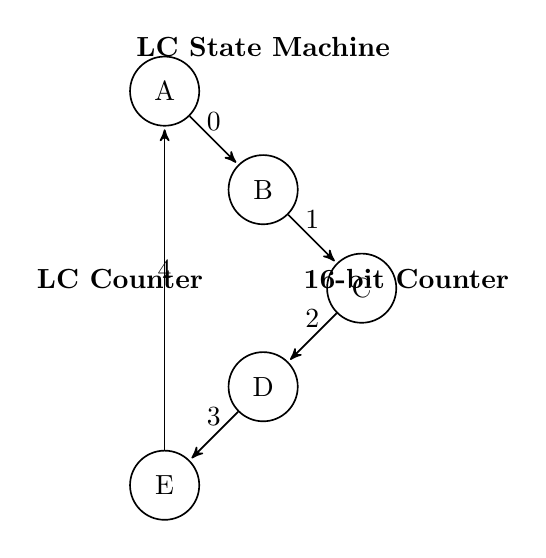
\begin{tikzpicture}[->,>=stealth',shorten >=1pt,auto,node distance=2cm,
                    semithick]
  \tikzstyle{every state}=[fill=white,draw=black,text=black]

  \matrix[row sep=1em, column sep=1em] {
    \node[state] (A) {A}; & & \\
    & \node[state] (B) {B}; & \\
    & & \node[state] (C) {C}; \\
    & \node[state] (D) {D}; & \\
    \node[state] (E) {E}; & & \\
  };

  \path (A) edge node[above] {0} (B)
        (B) edge node[above] {1} (C)
        (C) edge node[above] {2} (D)
        (D) edge node[above] {3} (E)
        (E) edge node[above] {4} (A);

  \node at (current bounding box.north) {\textbf{LC State Machine}};
  \node at (current bounding box.west) {\textbf{LC Counter}};
  \node at (current bounding box.east) {\textbf{16-bit Counter}};
\end{tikzpicture}

\end{document}